% This is "sig-alternate.tex" V2.1 April 2013
% This file should be compiled with V2.5 of "sig-alternate.cls" May 2012
%
% This example file demonstrates the use of the 'sig-alternate.cls'
% V2.5 LaTeX2e document class file. It is for those submitting
% articles to ACM Conference Proceedings WHO DO NOT WISH TO
% STRICTLY ADHERE TO THE SIGS (PUBS-BOARD-ENDORSED) STYLE.
% The 'sig-alternate.cls' file will produce a similar-looking,
% albeit, 'tighter' paper resulting in, invariably, fewer pages.
%
% ----------------------------------------------------------------------------------------------------------------
% This .tex file (and associated .cls V2.5) produces:
%       1) The Permission Statement
%       2) The Conference (location) Info information
%       3) The Copyright Line with ACM data
%       4) NO page numbers
%
% as against the acm_proc_article-sp.cls file which
% DOES NOT produce 1) thru' 3) above.
%
% Using 'sig-alternate.cls' you have control, however, from within
% the source .tex file, over both the CopyrightYear
% (defaulted to 200X) and the ACM Copyright Data
% (defaulted to X-XXXXX-XX-X/XX/XX).
% e.g.
% \CopyrightYear{2007} will cause 2007 to appear in the copyright line.
% \crdata{0-12345-67-8/90/12} will cause 0-12345-67-8/90/12 to appear in the copyright line.
%
% ---------------------------------------------------------------------------------------------------------------
% This .tex source is an example which *does* use
% the .bib file (from which the .bbl file % is produced).
% REMEMBER HOWEVER: After having produced the .bbl file,
% and prior to final submission, you *NEED* to 'insert'
% your .bbl file into your source .tex file so as to provide
% ONE 'self-contained' source file.
%
% ================= IF YOU HAVE QUESTIONS =======================
% Questions regarding the SIGS styles, SIGS policies and
% procedures, Conferences etc. should be sent to
% Adrienne Griscti (griscti@acm.org)
%
% Technical questions _only_ to
% Gerald Murray (murray@hq.acm.org)
% ===============================================================
%
% For tracking purposes - this is V2.0 - May 2012

\documentclass{sig-alternate}
\usepackage{hyperref}
\usepackage{graphicx}
\usepackage[font={large}]{caption}
\graphicspath{{images/}}

\begin{document}

% Copyright
%\setcopyright{acmcopyright}
%\setcopyright{acmlicensed}
\setcopyright{rightsretained}
%\setcopyright{usgov}
%\setcopyright{usgovmixed}
%\setcopyright{cagov}
%\setcopyright{cagovmixed}


% DOI
\doi{ }

% ISBN
\isbn{ }


%\acmPrice{\$15.00}

%
% --- Author Metadata here ---
\conferenceinfo{UofM:CoE:EECS}{2015, Ann Arbor MI}
%\CopyrightYear{2007} % Allows default copyright year (20XX) to be over-ridden - IF NEED BE.
%\crdata{0-12345-67-8/90/01}  % Allows default copyright data (0-89791-88-6/97/05) to be over-ridden - IF NEED BE.
% --- End of Author Metadata ---

\title{An Examination of B-Tree Performance in In-Memory Databases}
%\subtitle{An in-depth analysis}
%
% You need the command \numberofauthors to handle the 'placement
% and alignment' of the authors beneath the title.
%
% For aesthetic reasons, we recommend 'three authors at a time'
% i.e. three 'name/affiliation blocks' be placed beneath the title.
%
% NOTE: You are NOT restricted in how many 'rows' of
% "name/affiliations" may appear. We just ask that you restrict
% the number of 'columns' to three.
%
% Because of the available 'opening page real-estate'
% we ask you to refrain from putting more than six authors
% (two rows with three columns) beneath the article title.
% More than six makes the first-page appear very cluttered indeed.
%
% Use the \alignauthor commands to handle the names
% and affiliations for an 'aesthetic maximum' of six authors.
% Add names, affiliations, addresses for
% the seventh etc. author(s) as the argument for the
% \additionalauthors command.
% These 'additional authors' will be output/set for you
% without further effort on your part as the last section in
% the body of your article BEFORE References or any Appendices.

\numberofauthors{2} %  in this sample file, there are a *total*
% of EIGHT authors. SIX appear on the 'first-page' (for formatting
% reasons) and the remaining two appear in the \additionalauthors section.
%
\author{
% You can go ahead and credit any number of authors here,
% e.g. one 'row of three' or two rows (consisting of one row of three
% and a second row of one, two or three).
%
% The command \alignauthor (no curly braces needed) should
% precede each author name, affiliation/snail-mail address and
% e-mail address. Additionally, tag each line of
% affiliation/address with \affaddr, and tag the
% e-mail address with \email.
%
% 1st. author
\alignauthor
Isaac Bowen\\
       \affaddr{University of Michigan}
		\affaddr{College of Engineering}
		\affaddr{MSE: Computer Science and Engineering}
       \email{irbowen@umich.edu}
% 2nd. author
\alignauthor
Ryan Wawrzaszek\\
       \affaddr{University of Michigan}
		\affaddr{College of Engineering}
		\affaddr{MSE: Computer Science and Engineering}
       \email{ryanwawr@umich.edu}
}

\date{11 December 2015}
% Just remember to make sure that the TOTAL number of authors
% is the number that will appear on the first page PLUS the
% number that will appear in the \additionalauthors section.

\maketitle
\begin{abstract}
B-Trees are a fundamental structure for storing indexes in database systems. However, B-Trees were designed for use with systems and technology that are far different from the resources available to us today. In this project, we examine the performance of several different B-Tree implementations in order to gain an understanding of which elements of B-Trees are still valid for in-memory databases, and which elements need to be updated, removed, or replaced with structures more suited for use in modern database systems.
\end{abstract}

%
%  Use this command to print the description
%
%\printccsdesc

% We no longer use \terms command
%\terms{Theory}

%\keywords{ACM proceedings; \LaTeX; text tagging}
\keywords{B-Trees, Reader Writer Locks, B-Link}

\section{Introduction/Motivation}
Most traditional database management systems (DBMSs) use structures called B-Trees for storing indexes. B-Trees were designed to allow for efficient insertion and lookup of key-value pairs. However, this structure was developed decades ago, when DBMSs were run on single machines with small amounts of main memory, distributed applications were rare, and high availability was not a major concern. These circumstances influenced the design and structure of the B-Tree in critical ways, but database technology is a rapidly changing field. We have seen huge increases in processing power and main memory sizes, distributed applications have become commonplace, and clients have come to expect "always-on" systems with high availability for concurrent access. All of this means that many of the needs and assumptions that motivated the design of the B-Tree no longer hold true. 

Our particular focus in this paper is on the performance of B-Trees in in-memory databases. In the early days of relational databases, main memory was often too small to hold the full index. Therefore, B-Trees were designed to have a large fanout, since each level of the tree that had to be traversed incurred an additional disk I/O. Multi-threading was introduced to B-Trees, in part, to allow the processor to continue doing useful work while the next node of the tree was read into memory. Modern databases have advanced to the point where entire databases, even those containing several terabytes of information, can be stored in main memory. Our aim for this project was to analyze several different B-Tree implementations under an insert-heavy workload similar to those of modern OLTP databases.

\section{Previous Work}
B-trees have long been the primary access data structure for  relational databases. They have many properties that make them ideal structures for storing, retrieving, and using large amounts of data.\\
These include:
\begin{enumerate}
\item Efficient operations - Since all data is stored in the leaf nodes of the tree, the \texttt{update()} and \texttt{get()} operations only need to access one node at each level of the tree. Therefore, their runtime is logarithmic with respect to the fanout. The \texttt{insert()} operation is slightly more complex, as splits occurring in leaf nodes may propagate back up the tree, but the runtime is still logarithmic.
\item Maintaining elements in sorted order - In addition to allowing for efficient operations, maintaining elements in a sorted order allows for efficient joins on clustered indexes. Since selected tuples are retrieved in order, the sort-merge-join (SMJ) algorithm can be used without the expensive preprocessing step, allowing for improved query response times.
\item Block access - B-Trees often set the size of each node in the tree to be equivalent to the size of a memory page, adjusting the fan out of the system correspondingly in order to maximize space utilization. This also allows for efficient locking, as one needs only to lock the block id in order to lock the associated page. This made B-Tree's very popular early on, when most databases could not fit in memory, and had to be stored on disk.
\item Granular locking - B-Tree nodes can be locked individually. On each access, the DBMS only needs to lock the nodes that might be affected by the current operation. So long as the locking scheme maintains consistency within the tree, multiple threads are able to access the tree at once, improving concurrency and throughput.
\end{enumerate}

Many different structures and modifications of B-Trees have been proposed over the last 40 years.  In the original version of this data structure, data was stored in the inner nodes as well as in the leaf inner nodes.  This was seen as an optimal solution at the time as there was no wasted disk bandwidth, an important factor in an era when many DBMS applications were still single-threaded. A structure that limited data to the leaves would have wasted disk bandwidth by reading in a full page of data for each inner node, even though only the list of child nodes was needed. 

As applications became multi-threaded, new versions of the structure, such as B*Trees or B+Trees, switched to storing data exclusively in leaf nodes, storing only keys in the inner nodes. This loss of some amount of disk bandwidth associated with reading non-leaf nodes into memory was less critical in a multi-threaded environment. This shift in organization also allowed more keys to be stored in inner nodes, which gave trees a wider fanout and led to less total disk I/Os. Later versions of B-Trees also guaranteed that the tree structure was height balanced in order to provide good worst-case performance. They also added pointers linking leaf nodes together so that tables scans could be accomplished with only one traversal of the tree.  

Later implementations, such as that discussed in [2] added "sibling pointers" to inner nodes as well in an attempt to prolong splitting of nodes, which was a more expensive operation that a simple insert or retrieval. When a key was inserted into a node that would ordinarily be forced to split, it would instead check if it's sibling nodes had room for an additional key. If the sibling nodes were not full, keys were redistributed between the nodes in an order-preserving fashion. This allowed for delayed splitting of nodes and resulted in nodes that were, on average, closer to capacity. This served to minimize the depth of the tree which, in turn, decreased the amount of total disk I/Os needed to insert or retrieve a record.

Once DBMS applications moved to multi-threading, it became necessary to modify B-Trees to support concurrent access.  Several different locking schemes have been used in traditional B-Trees. The naive approach is to lock any node that could split on an insert.  It is impossible to know ahead of time which nodes will be accessed and which can potentially split, since, in a tree where each node is at full capacity, a split could propagate all the way up the tree to the root node. The simplest approach, then, is to acquire an exclusive lock on the root node before inserting, thereby locking the entire tree\cite{graefe:survey}. This is, in effect, no different from a single-threaded application, as no concurrency can be supported by this locking mechanics.

A slightly more refined locking mechanism involves acquiring a shared lock on the root node at the beginning of the operation. As the operation traverses the tree, it checks each node to see if it may be split by this operation. If it is determined that the child node cannot split, the shared lock is maintained. Otherwise, an exclusive lock must be acquired on both the child and parent nodes. This allows an increased degree of concurrency, as read operations can still proceed in a large portion of the tree while the insert takes place\cite{graefe:survey}\cite{lehman:locking}.  It should be noted, however, that this locking scheme can still lead to contention for a lock on the root node, especially in trees with small fanouts where nodes are split with a higher frequency.

\section{Our Approach}
We began by implementing a sequential access B-Tree with no locking mechanism and no support for concurrent access. This tree served as our baseline for measuring the performance of the concurrent access trees that we will discuss in Section 4. The sequential tree, as well as all other implementations, support the \texttt{insert()} and \texttt{get()} operations. We felt that this set of operations was sufficient to test our B-Tree implementations and locking mechanisms, as they provide the read and write functionality that will be needed to test our granular locking schemes.

We designed each B-Tree implementation in a manner that allows the fanout to be adjusted by setting a parameter. We were particularly interested in effect of node fanout on the performance of our implementations, given that the index and database are hosted entirely in main memory. Tree traversal is expensive for databases that are too large to fit in main memory, as a disk I/O is incurred every time a node is read in. This cost is not nearly as severe for an in-memory database, so we hypothesized that we would see less of a decrease in performance as fanout increased than would be observed in older databases.

We used the \texttt{std::rand()} function in C++ to generate key-value pairs for insertion and to determine whether an operation would be an insert or a retrieval. The percentage of reads and writes in the workload can be adjusted by means of an input parameter given to the program at runtime. We tested our implementations on insert-heavy workloads in order to simulate the workload of a modern OLTP database.

Given that our B-Tree implementations are intended for use in an in-memory database subject to insert-heavy workloads, we made several changes to the traditional B-Tree structure.  First, we do not we do not require the tree to be height-balanced.  Balanced trees are essential in DBMS applications for which the index and data are not hosted in memory, as a disk I/O is incurred for every level of the tree that is traversed. Therefore, balancing was required to limit disk I/O and provide reliable response times. For an in-memory database, however, the cost of "reading in" a node is merely the cost of following a pointer, so operation latencies are unlikely to vary significantly in an unbalanced tree. 

\begin{figure*}
	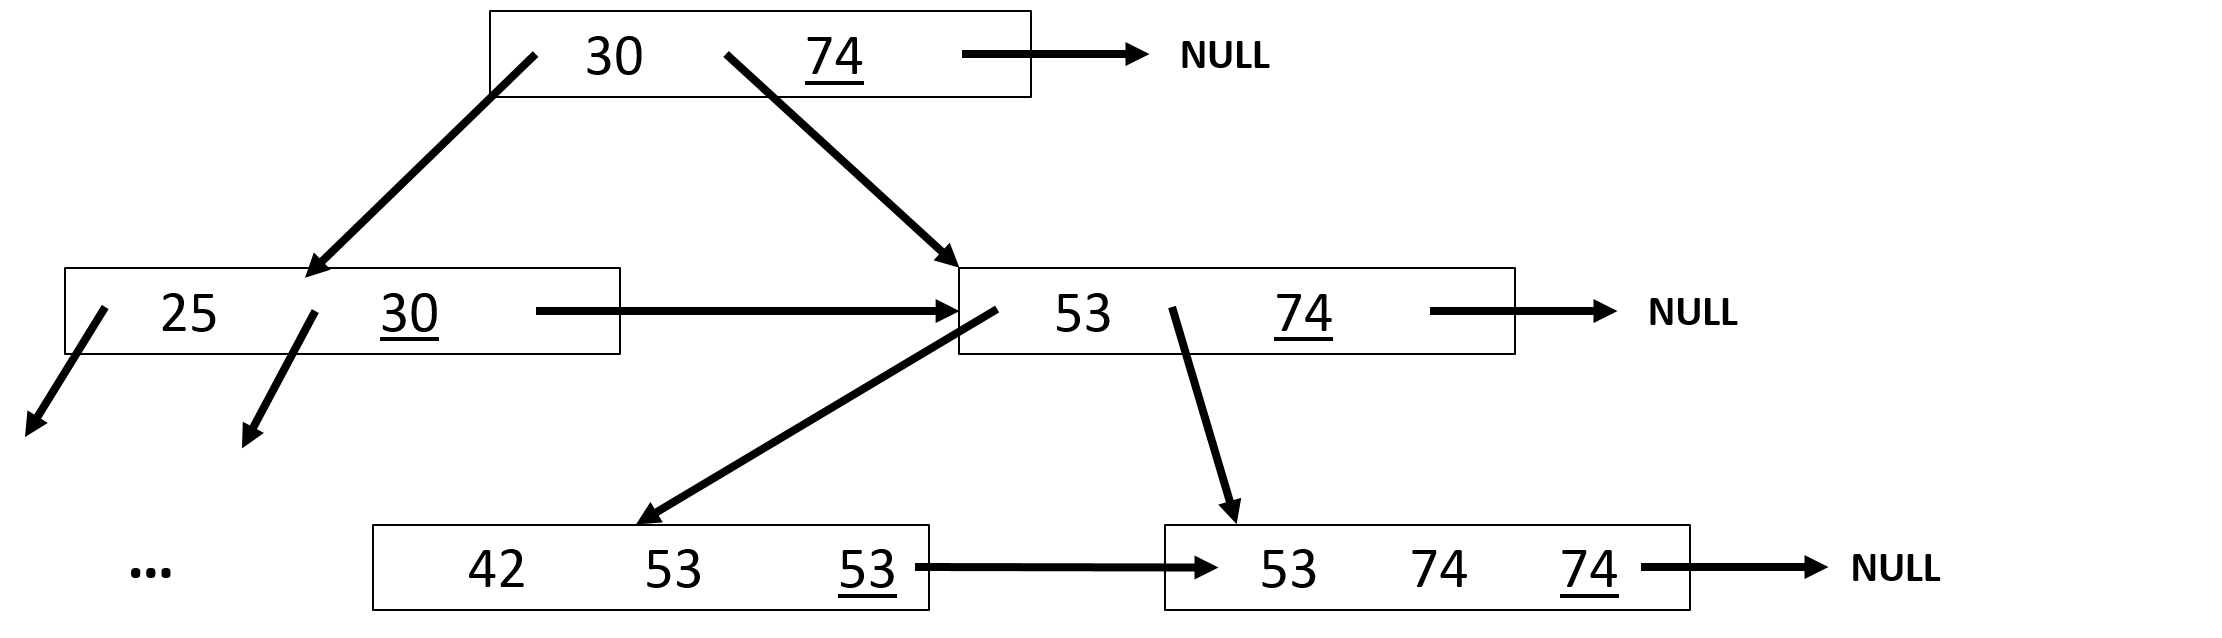
\includegraphics[width=\linewidth]{LinkTree}
	\caption[font={12}]{Example B-Link Tree. High keys are underlined.}
\end{figure*}

A balanced structure is a necessity for read-heavy workloads in which it is desirable to provide reliable latencies for lookups. It also allows for efficient scan operations, as the tree can be traversed from top to bottom once, then pointers joining leaf nodes can be followed in order to read in each element sequentially. However, maintaining this global depth can be expensive in a multi-threaded environment, as ensuring that nodes are linked and balanced in this fashion can incur significant locking overhead and cause a high amount of contention depending on how other relevant parameters of the tree are set.  We chose to abandon this requirement, and let the tree have varying depths of nodes.  This may increase slightly increase the time taken to locate the proper leaf node for an insertion or a lookup; however, the simpler locking protocol is likely to make up for this difference, as the cost of traversing the tree is quite low for an in-memory database, especially when compared to the cost incurred in a traditional database. 

Many B-Trees implement pointers to the neighboring nodes at the same level, for both leaf and inner nodes.  While this is certainly helpful for workloads containing a high percentage of range-based reads, maintaining these structures requires a cost to be paid on every insert.  In an insert-heavy workload, these small costs can add up quickly and have a much more significant impact on performance than they might have in more balanced workloads.  The potential performance benefits of maintaining these pointers relies on the tree being balanced.  Therefore, there is no reason to implement this aspect of the B-Tree in our sequential or ReaderWriter implementations. They are, however, maintained in the B-Link tree, as the "link pointers" are essential for proper locking.

\section{B-Tree Implementations}
The goal of our experiment is to observe the performance impact of varying each of the following parameters 
\begin{itemize}
  \item Input Size
  \item Locking Scheme
  \item Number of Threads
  \item Percentage of Insertions in Workload
  \item Fanout of Inner Nodes
\end{itemize}
In order to examine the performance of B-Trees in in-memory databases, we built four different tree implementations.
\subsection{Sequential Tree}
We began by building a simple, single-threaded B-tree to use as a baseline for testing.  The implementations discussed below build from this code, but implement various locking schemes to allow for concurrent access to the tree. There are three main classes used in the implementation - Tree, Inner\_Node, and Leaf\_Node.  The tree class manages the root node, which is always an Inner\_Node.  Both Inner\_Node and Leaf\_Node inherit from a Node, so they can call functions on their children without knowing what type of node they are.  Operations are generally executed by calling a function in the Tree class, which then calls the corresponding function in the root node.  The root node will then call the same function on the correct child, until the correct node has been found and the function can execute.
\subsection{ReaderWriter Trees (Array and List-based)}
This tree uses two different kinds of locks, shared and exclusive. As it traverses the tree, it checks to see whether the next child node can split, or whether it is a "safe" node. This implmentation is based on the idea's presented in \cite{lehman:locking}.

When an insert begins, the Tree class calls insert() on the root node.  The root node first acquires a shared lock, then scans through the node's keys, looking for the child node that the new key-value pair should be inserted into.  Once it has found the proper node, it checks to see if that node can split (i.e. whether that node is full).  If the child can split, then the parent upgrades to an exclusive lock, since, if the child splits, a new key will be pushed upwards in the tree and modify the parent's state. The exclusive lock prevents any other threads from inserting into that node or its children until the insert operation is complete and the lock is released.

This locking mechanism allows insert operations to hold shared reader locks in the top levels of the tree, upgrading to exclusive "writer" locks only when necessary. This allows for greater concurrency, as other threads can still perform read operations on other parts of the tree while the insertion takes place elsewhere.  However, locking a single node with an exclusive locks prevents any threads from inserting into that node or any of its children until the first insert operation has completed.

When a lookup begins, the Tree class calls the lookup() function on the root node. The root node acquires a shared lock, and then finds the correct child, just as it does for an insert. Once it finds the child, it simply calls the lookup function on that child and repeats the process.  This implementation ensures that multiple threads can read from the tree at concurrently. Lookup operations must block if they encounter a node for which an inserting thread holds an exclusive lock, waiting until that lock has been released before acquiring a shared lock and proceeding with the operation.

We create two different versions of the tree using reader writer locks - one that uses arrays to store the keys and values, and another that uses lists.  The two versions share most of the same code, the only major difference being the data underlying data structure that Inner\_Nodes use to store their children and that Leaf\_Nodes use to store their values.
\begin{figure*}
	\hspace{-15mm}
	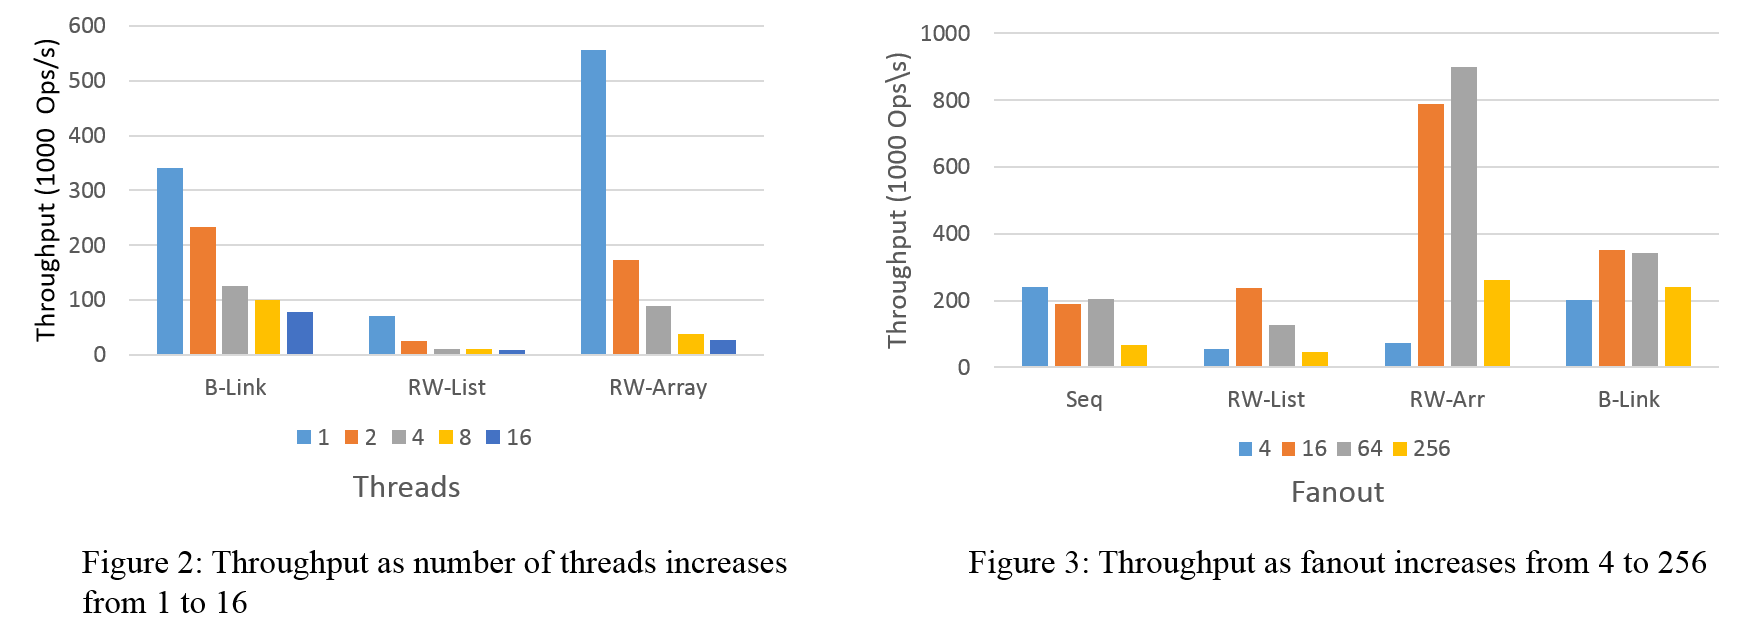
\includegraphics[width=200mm]{Figure34}
\end{figure*}

\subsection{B-Link Tree}
The B-Link tree is based on the work found in [3] and employs a bottom-up locking mechanism. The structure of the B-Link tree differs from that of a traditional tree in two main ways.

First, each node maintains a "link pointer" to the next node to the right at the same level. The pointer for the node furthest to the right is simply assigned a null value. These pointers appear as the horizontal arrows connecting nodes at the same level in Figure 1.

Second, each node maintains a "high key". The high key is the value of the highest key found in the subtree rooted at the node pointed to by the last non-link pointer in the node. High keys are depicted as underlined values in Figure 1.

These structural modifications allow for the implementation of a minimal and efficient locking scheme. On an insertion, each node accessed as the tree is traversed is pushed onto a stack, but is not locked. The first node to be locked is the leaf into which the new value is being inserted. If the insertion causes the node to exceed its capacity, the node is split. A link pointer is added from the original node to the new node, and the link pointer of the new node is set equal to the old link pointer of the original node.

Because the leaf's parent node does not know of the newly created leaf node, the two leaves can be considered one leaf, as the new node is essentially an extension of the original that can be reached by following the link pointer. The parent node is popped from the stack and locked. A pointer to the newly formed node is inserted, atomically adding the new node to the tree. At this point, the leaf node may be unlocked. If the parent node is forced to split, the same split procedure is followed. This continues up the tree until the split cannot propagate any further, at which point the last lock is released.

The search algorithm for the B-link tree is very similar to that of a traditional B-tree, but it acquires no locks. As the search travels down the tree, it scans each node to find the appropriate child to insert into. If the high key of the current node is less than the key being inserted, then this node has been split, and the search simply follows link pointers until it finds the node that contains a pointer to the proper child node.
\section{Implementation and Test Setup}
We implemented our B-Trees in \texttt{C++}, using new features only available in \texttt{C++14}, most notably \texttt{stdshared\_time\_mutex}, which allows both exclusive and shared locking.  This requires a compiler with \texttt{gc -4.9} or greater.  Because this is so new, few systems have made version 4.9 available. We were unable to update the compiler on \texttt{bigdata.eecs.umich.edu}, so we set up our own testing environment.

We set up a virtual machine using Oracle Virtual Box.  The VM is running Ubunutu Server 15.10 with gcc 4.9.3.  The host system is a Windows 7 machine with a FX-8350 (\texttt{8 cores @ 4Ghz}) and 32GB of RAM.  We allocated 4 cores and 24GB of RAM to the VM.  All test were run with minimal applications running on the Windows side.

We used \texttt{std::rand()} to generate input data.  


\section{Experimental Results}
In all of the figures below, Seq denotes the sequential access tree, B-Link denotes the B-Link Tree, RW-List denotes the list-based ReaderWriter Tree, and RW-Arr denotes the array-based ReaderWriter Tree. We measured performance by averaging the time taken to complete a specified number of operation, then calculating the throughput. The y-axis of each figure denotes throughput in thousands of operations completed per second. Specific conditions of each trial are given in the subsections that follow.

\subsection{Baseline Evaluation of Sequential Tree}
We began by testing our sequential tree on a variety of input sizes in order make sure that this implementation was efficient, since we planned to use it as a base for our concurrent versions.  We tested with various fan outs, namely 4, 16, 64, and 256.  We were surprised to see that performance degraded as the fan out increased.  We assumed that a larger node size would allow faster look-ups and inserts, because the operation would have to traverse fewer levels of the tree.  However,it seems that there is a difficult balance between traversal within a node, and traversal in the tree across nodes. This is discussed further in Section 6.3.

We observed that a fanout of 4 gave us the best performance for the sequential tree, so we decided to compare that to an in-memory tree.  We chose \texttt{std::map}, which is typically implemented using Red-black trees, as our basis for comparison.  When fan out was small, either 4 or 16, the performance of our sequential tree was better.  However, as the fan out increased, the performance of our implementation degraded to the point where it was somewhat slower than \texttt{std::map}. However, this performance gap was not large, so we proceeded to build our concurrent tree implementations.

\subsection{Analysis of Concurrency}
In order to analyze the effect of the B-Tree locking scheme and level of concurrency on performance, we measured throughput for a workload of 1,000,000 operations comprised of 90\% inserts and 10\% lookups. The fanout used for this experiment was 64.

We ran our code under these conditions varying the number of threads accessing the tree concurrently from 1 to 16 and averaging data from several trials. As is made clear in Figure 2, we observed a sharp decrease in performance as we increased the number of threads handling each workload. The decrease was most severe for the array-based ReaderWriter tree, which ran 20 times slower with 16 threads than it did when it was run as a single-threaded application.

This clear pattern indicates to us that concurrency is not a useful feature in an in-memory database run on a single server. This is hardly surprising, as one of the primary purposes of threading is to allow the processor to continue doing useful work while one thread is blocked waiting for a disk I/O to finish. Traditional databases tend to perform much better in a multi-threaded environment because they must block for disk I/O when reading in pages of records pointed to by leaf nodes as well as when reading in non-leaf nodes for databases where the index itself is too large to fit in memory. For an in-memory database such as our testing environment, however, there is no disk I/O associated with reading in an inner node or a leaf value. The cost, in our case, is simply that of following a pointer and reading the corresponding location in main memory. 

We believe that the performance decrease we observed in our trials can be attributed to the high and unnecessary overhead of the locking protocols used by our B-Tree implementations. The fact that the B-Link tree observed the least significant decrease in performance - a factor of 4, as compared to factors of 7 and 20 for the list-based and array-based implementations - supports this conclusion, since the locking protocol used in the B-Link tree should acquire far less locks during a typical tree traversal than either of the other implementations. Our results indicate that any possible benefits of a concurrent implementation in this environment are not nearly significant enough to offset the cost associated with the overhead of the locking protocol, which creates a good deal of resource contention that simply does not exist for single-threaded applications and which incurs context switches far more frequently. 

\subsection{Analysis of Fanout}
In order to analyze the effect of fanout on performance, we measured throughput for a workload of 1,000,000 operations comprised of 90\% inserts and 10\% lookups. We ran each trial as a single-threaded application, as our results above indicated that performance would be adversely affected by higher levels of concurrency.

We varied the fanout of each B-Tree implementation from 4 to 256 and averaged the throughput observed over the course of several trials to compile the results in Figure 3. For each of our three implementations, we observed a significant increase in performance when we increased the fanout from 4 to 16. Performance with a fanout of 64 was generally similar to the performance observed with a fanout of 16, but we observed a sharp decrease in performance once we increased the fanout parameter to 256. 

These findings are in opposition to what one would expect to see in a traditional database, in which performance tends to peak when fanout approaches 100, then levels off slowly. Our results are unsurprising, however, when considered in the context of an in-memory database. The initial increase in performance is most likely due to a sharp decrease in the number of splits occurring in the table. As fanout (and therefore node capacity) are increased, the frequency with which nodes are split will decrease sharply. This contributes to the sharp increase in throughput that we observed, as splitting nodes is a fairly expensive operation in comparison to other operations such as lookups and insertions that do not cause splits. 

We were harder pressed to explain why the drop off in performance that we observed when fanout was increased from 64 to 256 was so much more significant than what we would expect were we not operating with an in-memory database. We believe that this can be explained by the increased time required to search through each node and locate the pointer to the appropriate child. However, this cost would increase at exactly the same rate for a traditional database. 

The difference, we believe, is that, while increasing fanout serves to reduce the number of splits in both in-memory and traditional databases, it also serves the purpose of reducing disk I/O in traditional databases. Trees with larger fanouts are not as deep as those with lower fanouts, so less levels of the tree must be traversed by insert and lookup operations in order to locate the appropriate leaf node. In traditional databases, this reduces the number of disk I/Os required, which can provide significant performance benefits. As we stated in the previous subsection, there is no disk I/O required for any operations when the database is entirely in-memory. Therefore, we do not gain as much from having a shallow tree, and the performance decrease associated with searching though larger arrays of node pointers becomes more pronounced.

\vspace{3mm}
\hspace{-10mm}
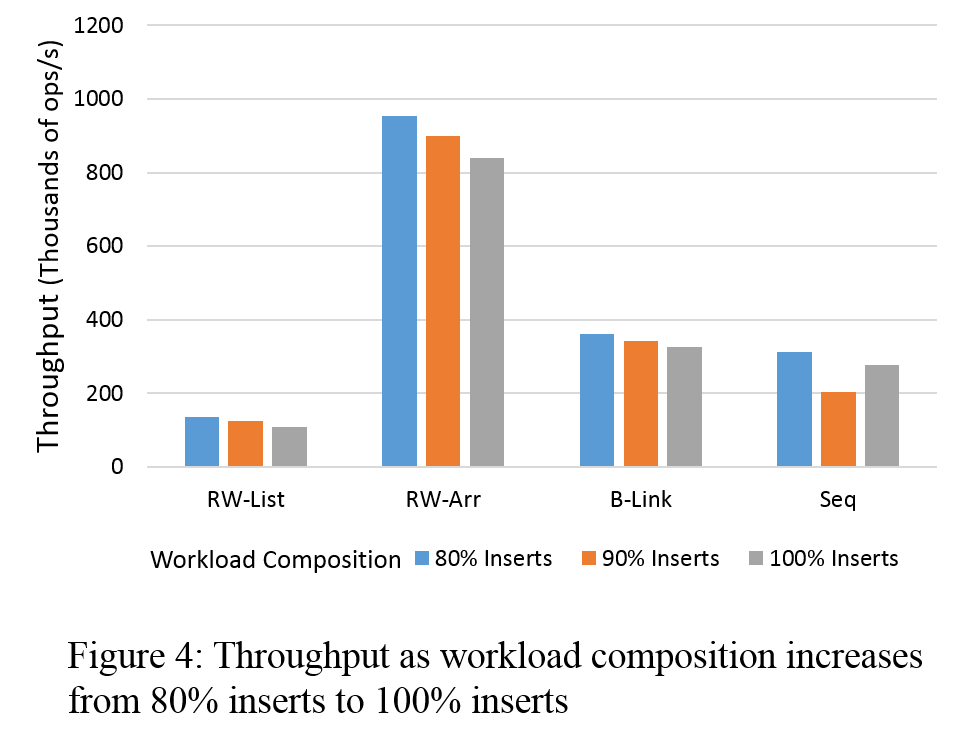
\includegraphics[width=\linewidth]{WorkloadGraph}
\vspace{3mm}

\subsection{Workload and Data Structure Analysis}
To analyze the effect of workload on performance, we ran trials of 1,000,000 operations with a fanout of 64. Results shown are for trials run as single-threaded applications. We varied the workload composition from 80\% insert operations to 100\% insert operations. Results are shown in Figure 4, above.

Our results showed a linear decrease in throughput as the percentage of insert operations in the workload increased.This increase was expected, as inserts are more expensive operations than lookups. One of our initial goals for this project was to determine which locking scheme would demonstrate the highest performance in a multi-threaded in-memory database. We believed that the B-Link tree would exhibit the best performance for insert-heavy workloads, as it's locking scheme requires it to acquire far fewer locks on average than the other implementations. Unfortunately, our multi-threaded workload tests showed similar trends but with significantly worse performance, as our earlier discussion on concurrency would suggest. 

That said, we were surprised to see that the array-based ReaderWriter tree exhibited throughput two to three times that of our other implementations. The standard array structure in the C++ standard library guarantees sequential location of the elements in memory, whereas the list structure simply maintains pointers to the next element. However, this is only a significant benefit when elements are being read from the disk, as random access in main memory is nearly as fast as sequential access. We suspect that caching is playing a role in the observed difference in throughput, as the elements of an array may be stored in one cache block if the fanout is small in comparison to the size of the cache blocks. List elements, on the other hand, may be spread out across several cache blocks, which could impact performance. Further examination of this performance differential is merited but is beyond the scope of this paper.

\section{Conclusion}
Several important lessons can be learned from this examination of B-Tree performance in in-memory databases.

\begin{itemize}
\item \textbf{Locking} The first, and perhaps the most critical conclusion we have drawn is that locking schemes have no place in in-memory databases. Our concurrent tree implementations performed very poorly in comparison to our sequential tree, even when run with only one thread. It is clear from the almost exponential performance decay we observed in our concurrency tests that the overhead and resource contention introduced by locking have a severe impact on performance.

B-Trees were originally designed for sequential rather than concurrent access, but as OS thread packages became more efficient and lightweight, concurrent access became a viable measure for improving performance. However, as Stonebraker observes in \cite{stone:oltp} and \cite{stone:era}. it is time for a rewrite of the system. Locking is expensive; the primary reason that locking schemes such as those we implemented were valuable in traditional databases is that disk I/O is even more expensive. Now, having freed ourselves of one bottleneck (disk I/O), it is time to free ourselves of another. Removing locking from B-Trees and reverting to single-threaded applications will make in-memory databases faster and will remove a great deal of complex code involved in safe locking protocols.

\item \textbf{Fanout} Varying fanout in an in our test environment revealed that there is a much more well-defined "sweet spot" for the fanout parameter in an in-memory database than there is in a traditional database. The cost of the disk I/Os associated with traversing a tree in a traditional database served to level the performance curve. For in-memory databases such as ours, there is a much more pronounced performance tradeoff between the frequency of splits and the number of values that must be iterated through to find the correct child pointer. We suspect that workload composition and fanout may be closely correlated, as both have a strong effect on the frequency with which nodes will be split. It seems that a study making a more detailed observation of the relationship between these two parameters would be beneficial.

\item \textbf{Vectors vs List} We decided to implement the array-based ReaderWriter tree at a fairly late stage of our project, but we are certainly glad that we did so, as this implementation consistently outperformed each of our other tree implementations, all of which make use of the C++ list as their underlying data structure. While we believe that caching or OS buffering may be playing a part in the observed benefits of using a structure that provides sequential memory addresses for its elements, we are not entirely certain what caused such a significant performance differential. We believe that it would be worthwhile to investigate this more closely in future projects.

\item \textbf{B-Tree vs Red black Tree} We observed that our sequential tree was able outperform \texttt{std::map} in most cases, but that, as the percentage of reads in the workload increased, \texttt{std::map}'s performance improved rapidly.  We believe that this is because we use an unbalanced B-Tree structure with high fan out (as compared to Red-Black Trees), which allows for faster inserts.  However, \texttt{std::map} must consistently perform re-balancing operations, which adds some overhead to the insert operation. This cost is offset by it's higher performance on read-heavy workloads, as it's structure allows for rapid lookups.

\end{itemize}

\section{Citations}
These papers provided a great deal of inspiration involved in the design of this experiment:
\begin{itemize}
  \item "Concurrent B-trees with Lock-free Techniques"\cite{sultana:lockfree} gave us the idea of implementing a lock free B-tree.  The implementation discussed in this paper, however, did not have access to the large memory and built-in C++14 atomics available to us. They also focused on trying to build a general purpose lock free btree for NUMA computers rather than studying insert-heavy workloads for in-memory databases. Unfortunately, we were unable to complete our implementation of the lock-free structure.
  \item "A survey of B-tree locking techniques"\cite{graefe:survey}, much like the title says, presents an overview of many of the different approaches that have been taken so far.
  \item "Efficient Locking for Concurrent Operations on B-Trees" \cite{lehman:locking} This paper provided the inspiration for the \texttt{can\_split()} function used in the ReaderWriter implementations and gave background on reader-writer locks.
\item "A Concurrent B-Link-Tree Algorithm Using a Cooperative Locking Protocol" \cite{lim:blink} This paper presented a modification of the B*-Tree that allowed for efficient locking, and provided us with details and background on the B-Link tree.
\end{itemize}

\bibliographystyle{plain}
\bibliography{mybib}

\end{document}
